\chapter{Results} %\label{Resultat}
The results of the simulations done in EnergyPlus and TRNSYS will be presented in this chapter.

\section{Energy demand}
To calculate the energy demand for space heating and cooling, an ideal air load is used and the simulation result from EnergyPlus is shown in figure \ref{fig:hd}. This figure shows the total heating and cooling load for each month and the average outdoor air dry bulb temperature. 

\begin{figure}[h!]
    \centering
    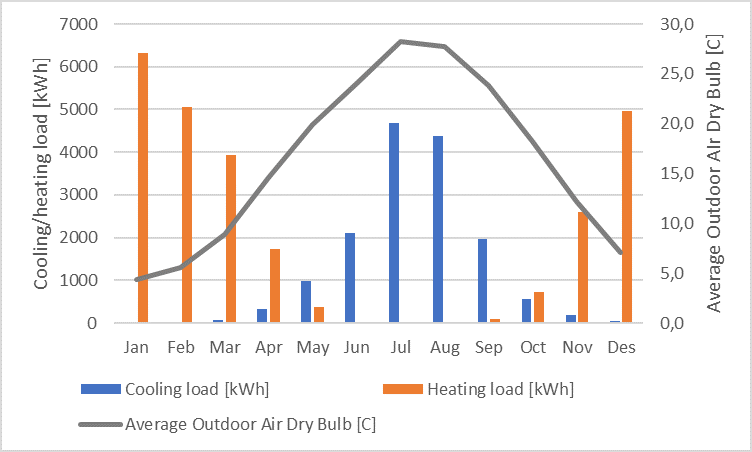
\includegraphics[scale=0.8]{vedlegg/combigraph.png}
    \caption{Heating load and cooling load vs average outdoor air dry bulb temperature, simulated in ENergyPlus}
    \label{fig:hd}
\end{figure}

Figure \ref{fig:ldch} displays hourly energy consumption for heating and cooling over a year. 

\begin{figure}[h!]
    \centering
    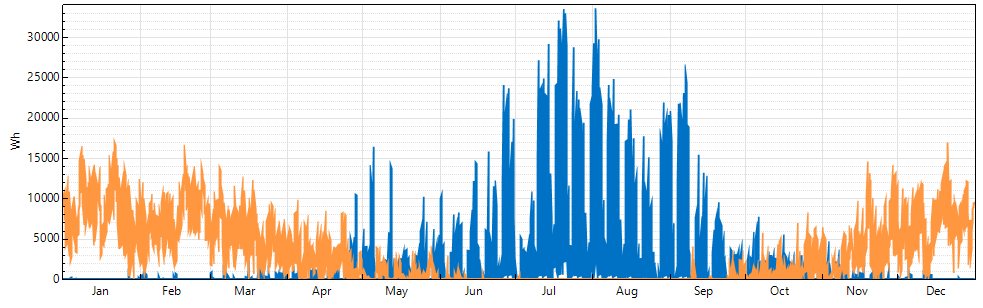
\includegraphics[scale=0.5]{vedlegg/coolheat.png}
    \caption{Energy consumption for heating and cooling, 1 hour time step.}
    \label{fig:ldch}
\end{figure}

Table \ref{tab:sum} gives a summary of the total energy demand for heating and cooling, the energy consumption per square meter and the peak load demand. 

\begin{table}[]
    \centering
        \caption{Summary of energy demand for space heating and cooling}
    \begin{tabular}{|p{2.5cm}|p{1.8cm}|p{1.8cm}|}
         \hline
        & \textbf{Heating} & \textbf{Cooling} \\
        \hline
        \textbf{Total energy demand [kWh]} & 25810.4 & 15321.0 \\
        \hline
        \textbf{kWh/m$^2$} & 61.5  & 36.5 \\
        \hline
        \textbf{Peak load [kW]} & 16.9 & 32.3 \\
        \hline
    \end{tabular}
    \label{tab:sum}
\end{table}

The hourly energy consumption from figure \ref{fig:ldch} gives a load duration curve for heating, figure \ref{fig:hload} and a load duration curve for cooling, figure \ref{fig:cload}.

\begin{figure}[h!]
    \centering
    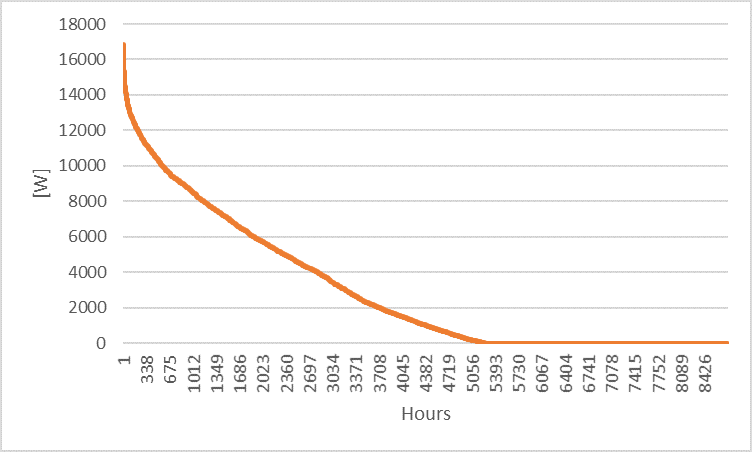
\includegraphics[scale=0.8]{vedlegg/hl1512.png}
    \caption{Load duration curve for space heating}
    \label{fig:hload}
\end{figure}

\begin{figure}[h!]
    \centering
    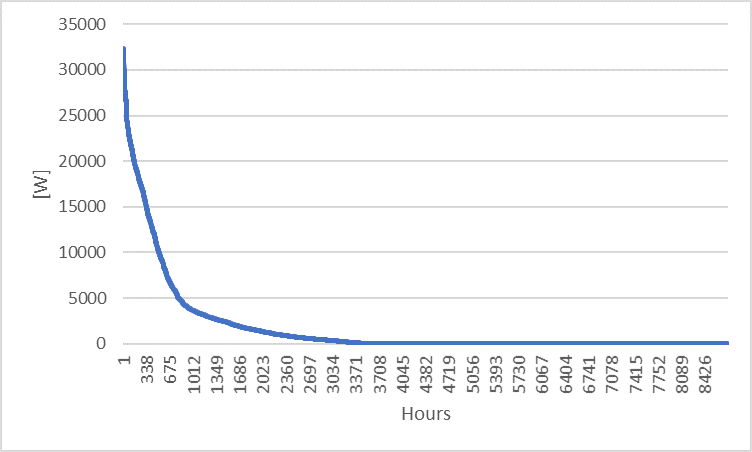
\includegraphics[scale=0.8]{vedlegg/cl1512.png}
    \caption{Load duration curve for space cooling}
    \label{fig:cload}
\end{figure}

\begin{table}[h!]
    \centering
       \caption{Caption}
    \begin{tabular}{|p{2cm}|p{2cm}|p{2cm}|p{2cm}|p{2cm}|p{2cm}|}
    \hline
        HP Capacity [kW] & Energy coverage Heating [\%]  & Energy coverage Cooling [\%] & Total energy coverage [\%] & Peak Load Coverage Heating [\%] & Peak Load Coverage Cooling [\%] \\
         \hline
          10 & 90.1 & 68.4 & 81.6 & 50.3& 27.0  \\
         \hline
         11 & 93.4 & 71.4 & 84.8 & 55.3 & 29.6   \\
         \hline
          12 & 95.8 & 74.3  & 87.4 &  60.3 & 32.3  \\
         \hline
          13 & 97.6 & 77.0 & 89.6 & 65.4 & 35.0 \\
         \hline
         14 & 98.8 & 79.5 & 91.3 & 70.3 & 37.7 \\
         \hline
         15 & 99.5 & 81.8 & 92.6 & 75.4 & 40.4  \\
         \hline
    \end{tabular}
    \label{tab:my_label}
\end{table}

An analysis of optimal angel for the PV panels was made and the result is displayed in figure \ref{fig:angel}. The result was an optimal angel of 22.5 degrees. 

\begin{figure}[h!]
    \centering
    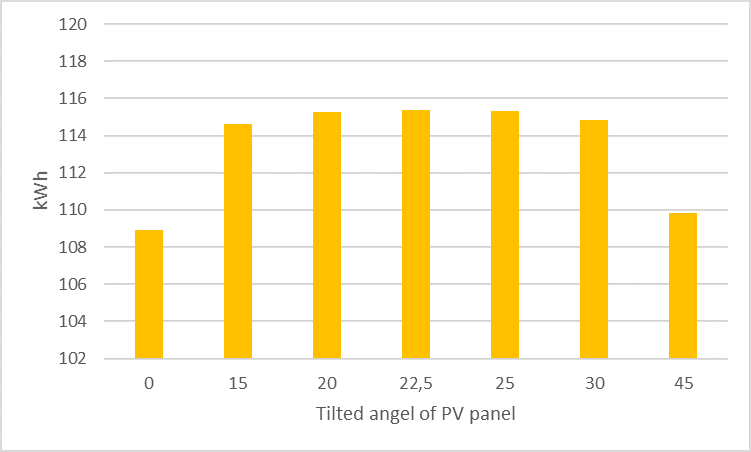
\includegraphics[scale=0.8]{vedlegg/angel.png}
    \caption{Analysis of optimal angel of PV panels, area = 0.89m$^2$, $\eta$ = 8.7\%}
    \label{fig:angel}
\end{figure}

\pagebreak

